\documentclass{article}
\usepackage{tikz}
\usepackage{pgfplots}
\usepackage{comment}
\usepackage{float,subfigure}
\usetikzlibrary{positioning}
\usetikzlibrary{arrows.meta}
\usetikzlibrary{calc}

\newcommand{\card}{\mathrm{card}}
\newcommand{\modrelu}{\sigma_{\mathrm{modReLU}, -1}}

\begin{document}
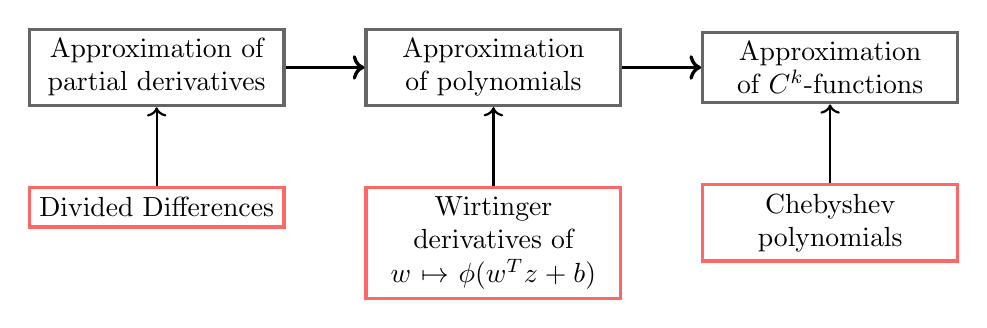
\begin{tikzpicture}[
roundnode/.style={circle, draw=green!60, fill=green!5, very thick, minimum size=7mm},
squarednode/.style={rectangle, draw=black!60,  very thick, minimum size=5mm, text width=3cm,align=center},
sidenode/.style={rectangle, draw=red!60,  very thick, minimum size=5mm, text width=3cm,align=center}
]
\node[squarednode]      (partialdev)                              {Approximation of partial derivatives};
\node[squarednode]        (polyn)       [right=of partialdev] {Approximation of polynomials};
\node[squarednode]      (ckfunctions)       [right=of polyn] {Approximation of $C^k$-functions};
\node[sidenode]            (divided_differences)  [below=of partialdev] {Divided Differences};
\node[sidenode]            (phi)  [below=of polyn] {Wirtinger derivatives of $w \mapsto \phi(w^T z + b)$};
\node[sidenode]            (cheby)  [below=of ckfunctions] {Chebyshev polynomials};

\draw[->, very thick] (partialdev.east) -- (polyn.west);
\draw[->, very thick] (polyn.east) -- (ckfunctions.west);
\draw[->, thick] (divided_differences.north) -- (partialdev.south);
\draw[->, thick] (phi.north) -- (polyn.south);
\draw[->, thick] (cheby.north) -- (ckfunctions.south);
\end{tikzpicture}

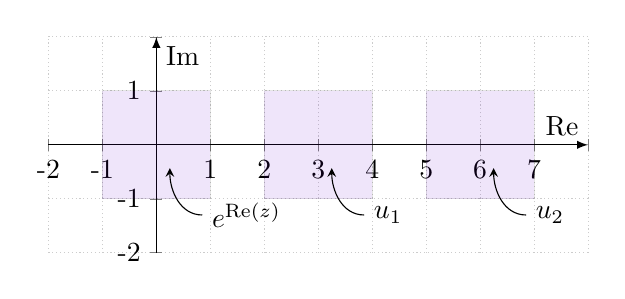
\begin{tikzpicture}
\begin{axis}[
  axis lines=middle,
  axis equal image,
  axis line style = {-latex},
  xmin=-2,xmax=8,ymin=-2,ymax=2,
  xtick distance = 1,
  ytick distance= 1,
  xticklabels = {\empty, -2, -1,0, 1,2,3,4,5,6,7,\empty},
  yticklabels = {\empty, -2 , -1, 0 , 1 , \empty},
  xlabel=Re,
  ylabel=Im,
  grid=major,
  grid style={thin,densely dotted,black!20}]
  \definecolor{mycolor}{RGB}{102,0,204}
 \draw[fill = mycolor, opacity = 0.1](axis cs:-1,-1) rectangle (axis cs: 1, 1) ;
 \draw[fill = mycolor, opacity = 0.1](axis cs: 2,-1) rectangle (axis cs: 4, 1) ;
  \draw[fill = mycolor, opacity = 0.1](axis cs: 5,-1) rectangle (axis cs: 7, 1) ;
  
  \node[anchor=west] (source1) at (axis cs:0.85, -1.3){ $e^{\mathrm{Re}(z)}$};
  \node (destination1) at (axis cs:0.25, -0.25){};
  \draw[->,>=stealth](source1) to [out=180,in=-90] (destination1);
  
  \node[anchor=west] (source2) at (axis cs:3.85, -1.3){ $u_1$};
  \node (destination2) at (axis cs:3.25, -0.25){};
  \draw[->,>=stealth](source2) to [out=180,in=-90] (destination2);
  
    \node[anchor=west] (source3) at (axis cs:6.85, -1.3){ $u_2$};
  \node (destination3) at (axis cs:6.25, -0.25){};
  \draw[->,>=stealth](source3) to [out=180,in=-90] (destination3);
\end{axis}
\end{tikzpicture}




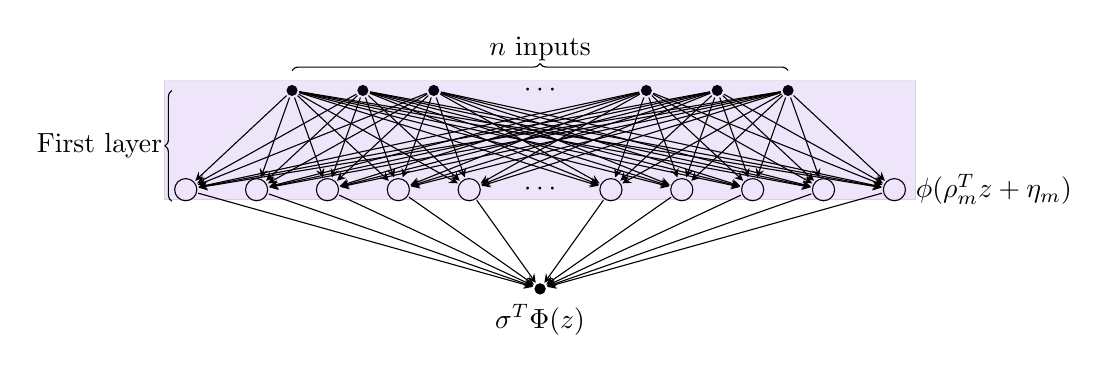
\begin{tikzpicture}[x=0.9cm,y=0.63cm,>=stealth,neuron/.style={circle,draw=black,inner sep=0pt,minimum size=8pt},
transition/.style={circle,fill=black,inner sep=0pt,minimum size=4pt},
pre/.style={->, shorten >=0.5pt,shorten <=0.5pt},
post/.style={->, shorten >=0.5pt,shorten <=0.5pt},
peri/.style={->, shorten >=0.5pt,shorten <=0.5pt}]

\node[transition] (init1) at (1,1){};
\node[transition] (init2) at (2,1){};
\node[transition] (init3) at (3,1){};
\node[transition] (init4) at (6,1){};
\node[transition] (init5) at (7,1){};
\node[transition] (init6) at (8,1){};
\node[neuron] (hidden1) at (-0.5,-1){};
\node[neuron] (hidden2) at (0.5,-1){};
\node[neuron] (hidden3) at (1.5,-1){};
\node[neuron] (hidden4) at (2.5,-1){};
\node[neuron] (hidden5) at (3.5,-1){};
\node[neuron] (hidden7) at (5.5,-1){};
\node[neuron] (hidden8) at (6.5,-1){};
\node[neuron] (hidden9) at (7.5,-1){};
\node[neuron] (hidden10) at (8.5,-1){};
\node[neuron,label=right:{$\phi(\rho_m^T z + \eta_m)$}] (hidden11) at (9.5,-1){};

\node[transition] (out) at (4.5,-3){};

\definecolor{mycolor}{RGB}{102,0,204}
\draw[fill = mycolor, opacity = 0.1](-0.8,-1.2) rectangle (9.8, 1.2) ;

\draw ($(init3)!0.5!(init4)$) node{$\cdots$};
\draw ($(hidden5)!0.5!(hidden7)$) node{$\cdots$};

\draw[pre](init1)--(hidden1);
\draw[pre](init1)--(hidden2);
\draw[pre](init1)--(hidden3);
\draw[pre](init1)--(hidden4);
\draw[pre](init1)--(hidden5);
\draw[pre](init1)--(hidden7);
\draw[pre](init1)--(hidden8);
\draw[pre](init1)--(hidden9);
\draw[pre](init1)--(hidden10);
\draw[pre](init1)--(hidden11);

\draw[pre](init2)--(hidden1);
\draw[pre](init2)--(hidden2);
\draw[pre](init2)--(hidden3);
\draw[pre](init2)--(hidden4);
\draw[pre](init2)--(hidden5);
\draw[pre](init2)--(hidden7);
\draw[pre](init2)--(hidden8);
\draw[pre](init2)--(hidden9);
\draw[pre](init2)--(hidden10);
\draw[pre](init2)--(hidden11);

\draw[pre](init3)--(hidden1);
\draw[pre](init3)--(hidden2);
\draw[pre](init3)--(hidden3);
\draw[pre](init3)--(hidden4);
\draw[pre](init3)--(hidden5);
\draw[pre](init3)--(hidden7);
\draw[pre](init3)--(hidden8);
\draw[pre](init3)--(hidden9);
\draw[pre](init3)--(hidden10);
\draw[pre](init3)--(hidden11);

\draw[pre](init4)--(hidden1);
\draw[pre](init4)--(hidden2);
\draw[pre](init4)--(hidden3);
\draw[pre](init4)--(hidden4);
\draw[pre](init4)--(hidden5);
\draw[pre](init4)--(hidden7);
\draw[pre](init4)--(hidden8);
\draw[pre](init4)--(hidden9);
\draw[pre](init4)--(hidden10);
\draw[pre](init4)--(hidden11);

\draw[pre](init5)--(hidden1);
\draw[pre](init5)--(hidden2);
\draw[pre](init5)--(hidden3);
\draw[pre](init5)--(hidden4);
\draw[pre](init5)--(hidden5);
\draw[pre](init5)--(hidden7);
\draw[pre](init5)--(hidden8);
\draw[pre](init5)--(hidden9);
\draw[pre](init5)--(hidden10);
\draw[pre](init5)--(hidden11);

\draw[pre](init6)--(hidden1);
\draw[pre](init6)--(hidden2);
\draw[pre](init6)--(hidden3);
\draw[pre](init6)--(hidden4);
\draw[pre](init6)--(hidden5);
\draw[pre](init6)--(hidden7);
\draw[pre](init6)--(hidden8);
\draw[pre](init6)--(hidden9);
\draw[pre](init6)--(hidden10);
\draw[pre](init6)--(hidden11);

\draw[post](hidden1)--(out);
\draw[post](hidden2)--(out);
\draw[post](hidden3)--(out);
\draw[post](hidden4)--(out);
\draw[post](hidden5)--(out);
\draw[post](hidden7)--(out);
\draw[post](hidden8)--(out);
\draw[post](hidden9)--(out);
\draw[post](hidden10)--(out);
\draw[post](hidden11)--(out);

 \draw [decoration={brace,raise=5pt},decorate] (init1.north) -- (init6.north) node [above=5pt,pos=0.5] {$n$ inputs};
  \draw [decoration={brace,raise=5pt, mirror},decorate] (-0.5,1) -- (hidden1.south) node [left=5pt,pos=0.5] {First layer};
  \node[transition, label=below:{$\sigma^T \Phi(z)$}] (out) at (4.5,-3){};
\end{tikzpicture}

\begin{tikzpicture}[x=0.9cm,y=0.63cm,>=stealth,neuron/.style={circle,draw=black,inner sep=0pt,minimum size=8pt},
transition/.style={circle,fill=black,inner sep=0pt,minimum size=4pt},
pre/.style={->, shorten >=0.5pt,shorten <=0.5pt},
post/.style={->, shorten >=0.5pt,shorten <=0.5pt},
peri/.style={->, shorten >=0.5pt,shorten <=0.5pt}]

\node[transition] (init1) at (1,-3){};
\node[transition] (init2) at (2,-3){};
\node[transition] (init3) at (3,-3){};
\node[transition] (init4) at (6,-3){};
\node[transition] (init5) at (7,-3){};
\node[transition] (init6) at (8,-3){};
\node[neuron,label={[xshift=-0.8cm, yshift=0cm]$\phi(\rho_m^T z + \eta_1)$}] (hidden11) at (-0.5,-1){};
\node[neuron] (hidden2) at (0.5,-1){};
\node[neuron] (hidden3) at (1.5,-1){};
\node[neuron] (hidden4) at (2.5,-1){};
\node[neuron] (hidden5) at (3.5,-1){};
\node[neuron] (hidden7) at (5.5,-1){};
\node[neuron] (hidden8) at (6.5,-1){};
\node[neuron] (hidden9) at (7.5,-1){};
\node[neuron] (hidden10) at (8.5,-1){};
\node[neuron,label={[xshift=0.8cm, yshift=0cm]$\phi(\rho_m^T z + \eta_m)$}] (hidden11) at (9.5,-1){};
\node[transition, label=above:{$\sigma^T \Phi(z)$}] (out) at (4.5,1){};

\definecolor{mycolor}{RGB}{102,0,204}
\draw[fill = mycolor, opacity = 0.1](-0.8,-3.1) rectangle (9.8, -0.75) ;

\draw ($(init3)!0.5!(init4)$) node{$\cdots$};
\draw ($(hidden5)!0.5!(hidden7)$) node{$\cdots$};

\draw[pre](init1)--(hidden1);
\draw[pre](init1)--(hidden2);
\draw[pre](init1)--(hidden3);
\draw[pre](init1)--(hidden4);
\draw[pre](init1)--(hidden5);
\draw[pre](init1)--(hidden7);
\draw[pre](init1)--(hidden8);
\draw[pre](init1)--(hidden9);
\draw[pre](init1)--(hidden10);
\draw[pre](init1)--(hidden11);

\draw[pre](init2)--(hidden1);
\draw[pre](init2)--(hidden2);
\draw[pre](init2)--(hidden3);
\draw[pre](init2)--(hidden4);
\draw[pre](init2)--(hidden5);
\draw[pre](init2)--(hidden7);
\draw[pre](init2)--(hidden8);
\draw[pre](init2)--(hidden9);
\draw[pre](init2)--(hidden10);
\draw[pre](init2)--(hidden11);

\draw[pre](init3)--(hidden1);
\draw[pre](init3)--(hidden2);
\draw[pre](init3)--(hidden3);
\draw[pre](init3)--(hidden4);
\draw[pre](init3)--(hidden5);
\draw[pre](init3)--(hidden7);
\draw[pre](init3)--(hidden8);
\draw[pre](init3)--(hidden9);
\draw[pre](init3)--(hidden10);
\draw[pre](init3)--(hidden11);

\draw[pre](init4)--(hidden1);
\draw[pre](init4)--(hidden2);
\draw[pre](init4)--(hidden3);
\draw[pre](init4)--(hidden4);
\draw[pre](init4)--(hidden5);
\draw[pre](init4)--(hidden7);
\draw[pre](init4)--(hidden8);
\draw[pre](init4)--(hidden9);
\draw[pre](init4)--(hidden10);
\draw[pre](init4)--(hidden11);

\draw[pre](init5)--(hidden1);
\draw[pre](init5)--(hidden2);
\draw[pre](init5)--(hidden3);
\draw[pre](init5)--(hidden4);
\draw[pre](init5)--(hidden5);
\draw[pre](init5)--(hidden7);
\draw[pre](init5)--(hidden8);
\draw[pre](init5)--(hidden9);
\draw[pre](init5)--(hidden10);
\draw[pre](init5)--(hidden11);

\draw[pre](init6)--(hidden1);
\draw[pre](init6)--(hidden2);
\draw[pre](init6)--(hidden3);
\draw[pre](init6)--(hidden4);
\draw[pre](init6)--(hidden5);
\draw[pre](init6)--(hidden7);
\draw[pre](init6)--(hidden8);
\draw[pre](init6)--(hidden9);
\draw[pre](init6)--(hidden10);
\draw[pre](init6)--(hidden11);

\draw[post](hidden1)--(out);
\draw[post](hidden2)--(out);
\draw[post](hidden3)--(out);
\draw[post](hidden4)--(out);
\draw[post](hidden5)--(out);
\draw[post](hidden7)--(out);
\draw[post](hidden8)--(out);
\draw[post](hidden9)--(out);
\draw[post](hidden10)--(out);
\draw[post](hidden11)--(out);

 \draw [decoration={brace,raise=5pt,mirror},decorate] (init1.south) -- (init6.south) node [below=5pt,pos=0.5] {$n$ inputs};
  \draw [decoration={brace,raise=5pt},decorate] (-0.5,-3) -- (hidden1.north) node [left=5pt,pos=0.5] {First layer};
\end{tikzpicture}

\end{document}
